\documentclass{article}

\usepackage{geometry}
\usepackage{amsmath}
\usepackage{graphicx}
\usepackage{listings}
\usepackage{hyperref}
\usepackage{multicol}
\usepackage{fancyhdr}
\pagestyle{fancy}
\hypersetup{ colorlinks=true, linkcolor=black, filecolor=magenta, urlcolor=cyan}
\geometry{ a4paper, total={170mm,257mm}, top=20mm, right=20mm, bottom=20mm, left=20mm}
\setlength{\parindent}{0pt}
\setlength{\parskip}{1em}
\renewcommand{\headrulewidth}{0pt}
\lhead{Competitive Programming - Arkavidia V}
\fancyfoot[CE,CO]{\thepage}

\begin{document}

\begin{center}
    \section*{D. DVD} % ganti judul soal

    \begin{tabular}{ | c c | }
        \hline
        Batas Waktu  & 1s \\    % jangan lupa ganti time limit
        Batas Memori & 64MB \\  % jangan lupa ganti memory limit
        \hline
    \end{tabular}
\end{center}

\subsection*{Deskripsi}

\begin{center}
    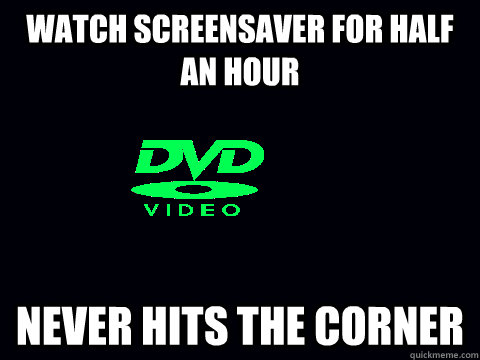
\includegraphics[width=200px]{meme}
\end{center}

Arvy sedang memandang layarnya yang berukuran $W \times H$ satuan.
Di layarnya, sedang berjalan \textit{screen saver} DVD.
Pada \textit{screen saver} ini, logo DVD bergerak lurus.
Ketika menyentuh sisi layar, logo DVD akan berubah warna dan memantul dengan sudut kedatangan sama dengan sudut pantulan (secara formal, sudut yang dibentuk antara garis gerakan logo sebelum memantul dan sisi layar sama dengan sudut yang dibentuk antara garis gerakan logo sesudah memantul dan sisi layar).
Setiap kali memantul, logo DVD berubah warna.

Arvy lelah menonton \textit{screen saver} DVD yang terus memantul-mantul.
Ia menunggu-nunggu kapan logo DVD berhenti di sudut layar.
Ia mulai ragu apakah logo DVD akan berhenti di sudut layar.
Akhirnya ia memfoto gerakan logo DVD dua kali, di mana logo DVD di kedua foto masih memiliki warna yang sama. Kedua logo ini berada di koordinat $(x_1, y_1)$ dan $(x_2, y_2)$.

\subsection*{Format Masukan}

Baris pertama terdiri dari satu bilangan bulat positif $T$ ($1 \leq T \leq 1.000$), menyatakan banyaknya kasus uji.

$T$ baris berikutnya terdiri dari 6 bilangan bulat, yakni $W$, $H$ ($1 \leq W, H \leq 1.000.000.000$), $x_1$, $y_1$, $x_2$, $y_2$ ($1 \leq x_1, x_2 \leq W$, $1 \leq y_1, y_2 \leq H$).

\subsection*{Format Keluaran}

Untuk tiap kasus uji, tuliskan \lstinline{YAY} jika logo DVD akan menyentuh koordinat tepat sudut layar TV, atau \lstinline{NAY} jika tidak.
\\

\begin{multicols}{2}
\subsection*{Contoh Masukan}
\begin{lstlisting}
3
5 5 1 2 2 3
6 3 3 3 4 2
6 5 6 3 3 2
\end{lstlisting}
\columnbreak
\subsection*{Contoh Keluaran}
\begin{lstlisting}
NAY
YAY
YAY
\end{lstlisting}
\vfill
\null
\end{multicols}

\subsection*{Penjelasan}
Untuk kasus uji pertama, layar TV dapat digambarkan seperti persegi panjang $ABCD$ di bawah, dengan posisi DVD pertama di titik $E$ dan posisi DVD kedua di titik $F$ disertai garis menunjukkan gerakan DVD. Jika ditelusuri, garis akan terus memantul dan tidak akan pernah sampai ke salah satu sudut.

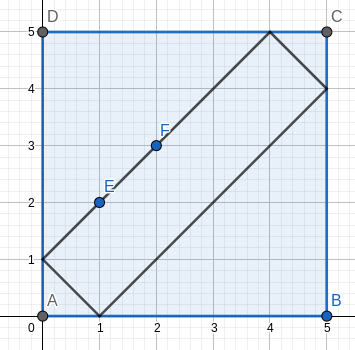
\includegraphics[height=150px]{sample-1}

Untuk kasus uji kedua, layar TV dapat digambarkan seperti persegi panjang $ABCD$ di bawah, dengan posisi DVD pertama di titik $E$ dan posisi DVD kedua di titik $F$ disertai garis menunjukkan gerakan DVD.

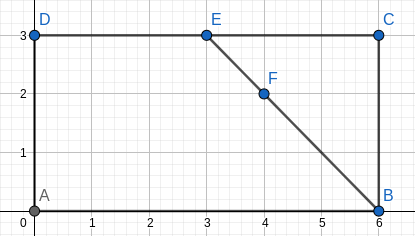
\includegraphics[height=150px]{sample-2}

Untuk kasus uji ketiga, layar TV dapat digambarkan seperti persegi panjang $ABCD$ di bawah, dengan posisi DVD pertama di titik $E$ dan posisi DVD kedua di titik $F$ disertai garis menunjukkan gerakan DVD.

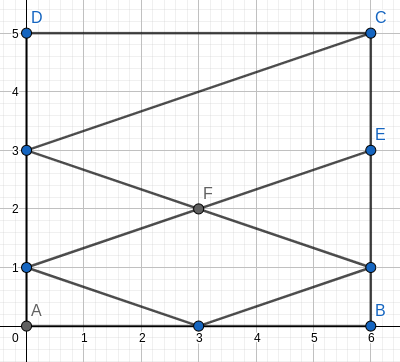
\includegraphics[height=150px]{sample-3}

\pagebreak

\end{document}